\documentclass[11pt]{article}
\usepackage{geometry}
\geometry{letterpaper}

\usepackage{graphicx}
\usepackage{amssymb}
\usepackage{float}
\usepackage{tabularx}
\usepackage{multicol}
\usepackage{hyperref}
\hypersetup{
    colorlinks,
    citecolor=black,
    filecolor=blue,
    linkcolor=black,
    urlcolor=black
}

% TODOs:
% ask Nick about lines in Seq Diagram, ask Nick about need 3D model, ask Nick about entering project goals
% switch to cleveref

\begin{document}

\begin{titlepage}
	\newcommand{\HRule}{\rule{\linewidth}{0.2mm}}
	\begin{center}
	\textsc{\LARGE McMaster University}\\[1.5cm]

	\textsc{\Large SmartServe}\\[0.5cm]
	\textsc{\large Software \& Mechatronics Capstone}\\[0.5cm]

	\HRule\\[0.4cm]
		{\huge\bfseries Low Level System Design}\\[0.4cm]
	\HRule\\[0.4cm]

	\begin{minipage}[t][][t]{0.5\textwidth}
		\begin{flushleft} \large
			\emph{Authors:}\\
			Christopher McDonald\\
			Harit Patel \\
			Janak Patel \\
			Jared Rayner  \\
			Nisarg Patel  \\
			Sam Hamel \\
			Sharon Platkin \\
		\end{flushleft}
	\end{minipage}
	~
	\begin{minipage}[t][][t]{0.4\textwidth}
		\begin{flushright} \large
			\emph{Professor:} \\
			Dr. Alan Wassyng \\[0.4cm]
			\emph{Teaching Assistants:} \\
			Bennett Mackenzie \\
			Nicholas Annable \\
			Stephen Wynn-Williams \\
			Viktor Smirnov
		\end{flushright}
	\end{minipage}\\[2cm]

	
\includegraphics[width=0.3\textwidth]{../logo.png} \\
	{\large Last compiled on \today}
	\end{center}

\end{titlepage}

\tableofcontents
\listoffigures

\vfill
\begin{figure}[H]
   \centering
   \noindent\begin{tabularx}{\textwidth}{| >{\centering\arraybackslash}m{0.2\textwidth} | >{\centering\arraybackslash}m{0.2\textwidth} | >{\centering\arraybackslash}m{0.2\textwidth} | >{\centering\arraybackslash}m{0.285\textwidth} |}
   \hline
   \textbf{Date} & \textbf{Revision} & \textbf{Comments} & \textbf{Author(s)} \\ \hline
   Dec ?, 2017 & 1.0 & Main content done for all sections & Christopher McDonald \\ \hline
   \end{tabularx}
   \caption{Revision History}
\end{figure}
\newpage
\section{Introduction}
\subsection{Project Overview}
SmartServe is an autonomous table tennis training system for table tennis players with various skill levels. SmartServe aids in diagnosing and improving a player's performance over time. The system trains table tennis players by shooting table tennis balls towards the player and detects successful returns from the player. The system can further adapt to the player's weaknesses and help them overcome it through further training. Importantly, SmartServe alleviates the problems of finding and working with a coach for players, as well as coaches trying to train multiple players simultaneously. The system will be deemed a success if the table tennis players and coaches can enjoy and see some value added by using SmartServe.\\\\
The project started at the beginning of the Fall 2017 academic term and will conclude at the end of the Winter 2018 term. In addition, the core project team consists of final year Software and Mechatronics Engineering students who are enrolled in the MECHTRON 4TB6/SFWRENG 4G06 capstone project course.
\subsection{Document Overview}
\subsection{Naming Conventions and Terminology}
\label{sec:definitions}
The following terms and definitions will be used throughout this document:
\begin{itemize}
% Alphabetical order is highly preferred as it eases user navigation
\item \textbf{ACID}: a database transaction which is atomic, consistent, isolated and durable
\item \textbf{CV}: computer vision
\item \textbf{FPS}: frames per second
\item \textbf{FSM}: finite state machine, shows transitions between states
\item \textbf{GUI}: graphical user interface
\item \textbf{IPO}: input process output
\item \textbf{Pitch}: rotation along the y-axis; this rotation angle primarily dictates the range of the ball from the net to the edge of the table on the user side
\item \textbf{Roll}: rotation along the x-axis
\item \textbf{Shooting Mechanism}: refers to the part of the system that shoots the table tennis balls towards the user side (player) Please refer to Figure \ref{fig:table-tennis-top-view} for visual illustration
\item \textbf{System}: encompasses both the hardware and software parts of SmartServe
\item \textbf{System Side}: the side of the table where the electromechanical system is placed; it is the opposite side of the User Side Please refer to Figure \ref{fig:table-tennis-top-view} for visual illustration
\item \textbf{TCP:} transmission control protocol
\item \textbf{Team}: all team members of the core capstone project, as noted in the list of Authors
\item \textbf{User Side}: the side of the table where the user (player) is standing
\item \textbf{Yaw}: rotation along the z-axis; this rotation angle primarily dictates the panning functionality of the shooting mechanism from the right side to the left side of the table
\end{itemize}

\begin{figure}[H]
   \centering
   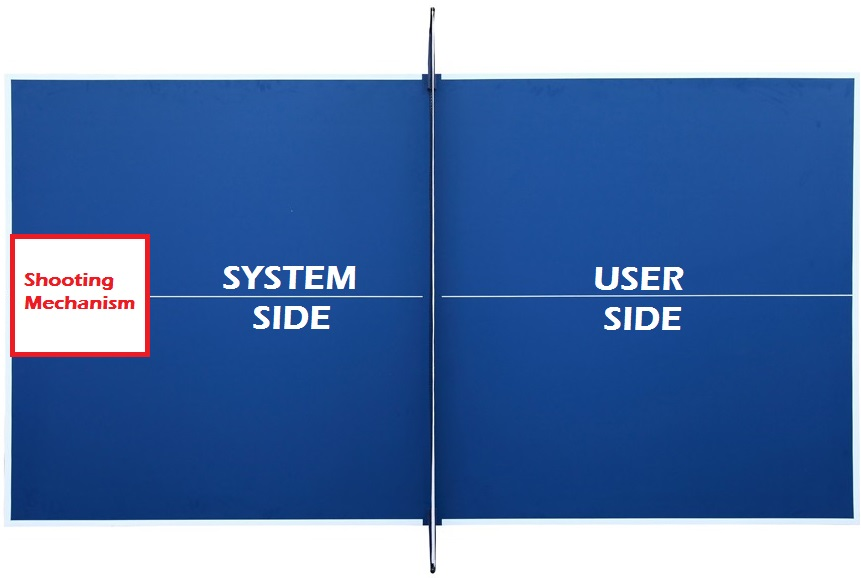
\includegraphics[width=0.75\textwidth]{../img/Table-Tennis-Top-View.png} %requires the graphicx package
   \caption{Top View of the Tennis Table}
   \label{fig:table-tennis-top-view}
\end{figure}

\section{Detailed Class Diagram}

\section{Module Guide}
\subsection{SmartServe Modules}
\subsubsection*{Module 1}
\textbf{Responsibilities} \\
some text \\
\textbf{Secrets} \\ 
some text \\ 
\textbf{MID} \\
some text \\
\textbf{MIS} \\
some text \\
\subsection{Shot Recommendation Modules}
\subsubsection*{Module 1}
\textbf{Responsibilities} \\
some text \\
\textbf{Secrets} \\ 
some text \\ 
\textbf{MID} \\
some text \\
\textbf{MIS} \\
some text \\
\subsection{Shooting Model Modules}
\subsubsection*{Module 1}
\textbf{Responsibilities} \\
some text \\
\textbf{Secrets} \\ 
some text \\ 
\textbf{MID} \\
some text \\
\textbf{MIS} \\
some text \\
\subsection{Shot Optimizer Modules}
\subsubsection*{Module 1}
\textbf{Responsibilities} \\
some text \\
\textbf{Secrets} \\ 
some text \\ 
\textbf{MID} \\
some text \\
\textbf{MIS} \\
some text \\
\subsection{Computer Vision Modules}
\subsubsection*{Module 1}
\textbf{Responsibilities} \\
some text \\
\textbf{Secrets} \\ 
some text \\ 
\textbf{MID} \\
some text \\
\textbf{MIS} \\
some text \\
\subsection{Data Storage Modules}
\subsubsection*{Module 1}
\textbf{Responsibilities} \\
some text \\
\textbf{Secrets} \\ 
some text \\ 
\textbf{MID} \\
some text \\
\textbf{MIS} \\
some text \\
\subsection{Shooting Mechanism Modules}
\subsubsection*{Module 1}
\textbf{Responsibilities} \\
some text \\
\textbf{Secrets} \\ 
some text \\ 
\textbf{MID} \\
some text \\
\textbf{MIS} \\
some text \\
\subsection{User Interface Modules}
\subsubsection*{Module 1}
\textbf{Responsibilities} \\
some text \\
\textbf{Secrets} \\ 
some text \\ 
\textbf{MID} \\
some text \\
\textbf{MIS} \\
some text \\

\section{Communication Protocols}
\subsection{Smart Serve to Shot Recommendation}
\subsection{Smart Serve to Shooting Mechanism}
\subsection{Smart Serve to Computer Vision}
\subsection{Smart Serve to User Interface}
\subsection{Smart Serve to Shot Optimizer}
\subsection{Smart Serve to Shooting Model}
\subsection{Smart Serve to Data Storage}
\subsection{Shot Recommendation to Data Storage}




\end{document}
